% Options for packages loaded elsewhere
% Options for packages loaded elsewhere
\PassOptionsToPackage{unicode}{hyperref}
\PassOptionsToPackage{hyphens}{url}
\PassOptionsToPackage{dvipsnames,svgnames,x11names}{xcolor}
%
\documentclass[
  ignorenonframetext,
  aspectratio=169,
  xcolor=\{dvipsnames\}]{beamer}
\newif\ifbibliography
\usepackage{pgfpages}
\setbeamertemplate{caption}[numbered]
\setbeamertemplate{caption label separator}{: }
\setbeamercolor{caption name}{fg=normal text.fg}
\beamertemplatenavigationsymbolsempty
% remove section numbering
\setbeamertemplate{part page}{
  \centering
  \begin{beamercolorbox}[sep=16pt,center]{part title}
    \usebeamerfont{part title}\insertpart\par
  \end{beamercolorbox}
}
\setbeamertemplate{section page}{
  \centering
  \begin{beamercolorbox}[sep=12pt,center]{section title}
    \usebeamerfont{section title}\insertsection\par
  \end{beamercolorbox}
}
\setbeamertemplate{subsection page}{
  \centering
  \begin{beamercolorbox}[sep=8pt,center]{subsection title}
    \usebeamerfont{subsection title}\insertsubsection\par
  \end{beamercolorbox}
}
% Prevent slide breaks in the middle of a paragraph
\widowpenalties 1 10000
\raggedbottom
\AtBeginPart{
  \frame{\partpage}
}
\AtBeginSection{
  \ifbibliography
  \else
    \frame{\sectionpage}
  \fi
}
\AtBeginSubsection{
  \frame{\subsectionpage}
}
\usepackage{iftex}
\ifPDFTeX
  \usepackage[T1]{fontenc}
  \usepackage[utf8]{inputenc}
  \usepackage{textcomp} % provide euro and other symbols
\else % if luatex or xetex
  \usepackage{unicode-math} % this also loads fontspec
  \defaultfontfeatures{Scale=MatchLowercase}
  \defaultfontfeatures[\rmfamily]{Ligatures=TeX,Scale=1}
\fi

\usetheme[]{Madrid}
\usepackage[]{libertinus}
\ifPDFTeX\else
  % xetex/luatex font selection
\fi
% Use upquote if available, for straight quotes in verbatim environments
\IfFileExists{upquote.sty}{\usepackage{upquote}}{}
\IfFileExists{microtype.sty}{% use microtype if available
  \usepackage[]{microtype}
  \UseMicrotypeSet[protrusion]{basicmath} % disable protrusion for tt fonts
}{}
\makeatletter
\@ifundefined{KOMAClassName}{% if non-KOMA class
  \IfFileExists{parskip.sty}{%
    \usepackage{parskip}
  }{% else
    \setlength{\parindent}{0pt}
    \setlength{\parskip}{6pt plus 2pt minus 1pt}}
}{% if KOMA class
  \KOMAoptions{parskip=half}}
\makeatother

\usepackage{color}
\usepackage{fancyvrb}
\newcommand{\VerbBar}{|}
\newcommand{\VERB}{\Verb[commandchars=\\\{\}]}
\DefineVerbatimEnvironment{Highlighting}{Verbatim}{commandchars=\\\{\}}
% Add ',fontsize=\small' for more characters per line
\usepackage{framed}
\definecolor{shadecolor}{RGB}{241,243,245}
\newenvironment{Shaded}{\begin{snugshade}}{\end{snugshade}}
\newcommand{\AlertTok}[1]{\textcolor[rgb]{0.68,0.00,0.00}{#1}}
\newcommand{\AnnotationTok}[1]{\textcolor[rgb]{0.37,0.37,0.37}{#1}}
\newcommand{\AttributeTok}[1]{\textcolor[rgb]{0.40,0.45,0.13}{#1}}
\newcommand{\BaseNTok}[1]{\textcolor[rgb]{0.68,0.00,0.00}{#1}}
\newcommand{\BuiltInTok}[1]{\textcolor[rgb]{0.00,0.23,0.31}{#1}}
\newcommand{\CharTok}[1]{\textcolor[rgb]{0.13,0.47,0.30}{#1}}
\newcommand{\CommentTok}[1]{\textcolor[rgb]{0.37,0.37,0.37}{#1}}
\newcommand{\CommentVarTok}[1]{\textcolor[rgb]{0.37,0.37,0.37}{\textit{#1}}}
\newcommand{\ConstantTok}[1]{\textcolor[rgb]{0.56,0.35,0.01}{#1}}
\newcommand{\ControlFlowTok}[1]{\textcolor[rgb]{0.00,0.23,0.31}{\textbf{#1}}}
\newcommand{\DataTypeTok}[1]{\textcolor[rgb]{0.68,0.00,0.00}{#1}}
\newcommand{\DecValTok}[1]{\textcolor[rgb]{0.68,0.00,0.00}{#1}}
\newcommand{\DocumentationTok}[1]{\textcolor[rgb]{0.37,0.37,0.37}{\textit{#1}}}
\newcommand{\ErrorTok}[1]{\textcolor[rgb]{0.68,0.00,0.00}{#1}}
\newcommand{\ExtensionTok}[1]{\textcolor[rgb]{0.00,0.23,0.31}{#1}}
\newcommand{\FloatTok}[1]{\textcolor[rgb]{0.68,0.00,0.00}{#1}}
\newcommand{\FunctionTok}[1]{\textcolor[rgb]{0.28,0.35,0.67}{#1}}
\newcommand{\ImportTok}[1]{\textcolor[rgb]{0.00,0.46,0.62}{#1}}
\newcommand{\InformationTok}[1]{\textcolor[rgb]{0.37,0.37,0.37}{#1}}
\newcommand{\KeywordTok}[1]{\textcolor[rgb]{0.00,0.23,0.31}{\textbf{#1}}}
\newcommand{\NormalTok}[1]{\textcolor[rgb]{0.00,0.23,0.31}{#1}}
\newcommand{\OperatorTok}[1]{\textcolor[rgb]{0.37,0.37,0.37}{#1}}
\newcommand{\OtherTok}[1]{\textcolor[rgb]{0.00,0.23,0.31}{#1}}
\newcommand{\PreprocessorTok}[1]{\textcolor[rgb]{0.68,0.00,0.00}{#1}}
\newcommand{\RegionMarkerTok}[1]{\textcolor[rgb]{0.00,0.23,0.31}{#1}}
\newcommand{\SpecialCharTok}[1]{\textcolor[rgb]{0.37,0.37,0.37}{#1}}
\newcommand{\SpecialStringTok}[1]{\textcolor[rgb]{0.13,0.47,0.30}{#1}}
\newcommand{\StringTok}[1]{\textcolor[rgb]{0.13,0.47,0.30}{#1}}
\newcommand{\VariableTok}[1]{\textcolor[rgb]{0.07,0.07,0.07}{#1}}
\newcommand{\VerbatimStringTok}[1]{\textcolor[rgb]{0.13,0.47,0.30}{#1}}
\newcommand{\WarningTok}[1]{\textcolor[rgb]{0.37,0.37,0.37}{\textit{#1}}}

\usepackage{longtable,booktabs,array}
\usepackage{calc} % for calculating minipage widths
\usepackage{caption}
% Make caption package work with longtable
\makeatletter
\def\fnum@table{\tablename~\thetable}
\makeatother
\usepackage{graphicx}
\makeatletter
\newsavebox\pandoc@box
\newcommand*\pandocbounded[1]{% scales image to fit in text height/width
  \sbox\pandoc@box{#1}%
  \Gscale@div\@tempa{\textheight}{\dimexpr\ht\pandoc@box+\dp\pandoc@box\relax}%
  \Gscale@div\@tempb{\linewidth}{\wd\pandoc@box}%
  \ifdim\@tempb\p@<\@tempa\p@\let\@tempa\@tempb\fi% select the smaller of both
  \ifdim\@tempa\p@<\p@\scalebox{\@tempa}{\usebox\pandoc@box}%
  \else\usebox{\pandoc@box}%
  \fi%
}
% Set default figure placement to htbp
\def\fps@figure{htbp}
\makeatother


% definitions for citeproc citations
\NewDocumentCommand\citeproctext{}{}
\NewDocumentCommand\citeproc{mm}{%
  \begingroup\def\citeproctext{#2}\cite{#1}\endgroup}
\makeatletter
 % allow citations to break across lines
 \let\@cite@ofmt\@firstofone
 % avoid brackets around text for \cite:
 \def\@biblabel#1{}
 \def\@cite#1#2{{#1\if@tempswa , #2\fi}}
\makeatother
\newlength{\cslhangindent}
\setlength{\cslhangindent}{1.5em}
\newlength{\csllabelwidth}
\setlength{\csllabelwidth}{3em}
\newenvironment{CSLReferences}[2] % #1 hanging-indent, #2 entry-spacing
 {\begin{list}{}{%
  \setlength{\itemindent}{0pt}
  \setlength{\leftmargin}{0pt}
  \setlength{\parsep}{0pt}
  % turn on hanging indent if param 1 is 1
  \ifodd #1
   \setlength{\leftmargin}{\cslhangindent}
   \setlength{\itemindent}{-1\cslhangindent}
  \fi
  % set entry spacing
  \setlength{\itemsep}{#2\baselineskip}}}
 {\end{list}}
\usepackage{calc}
\newcommand{\CSLBlock}[1]{\hfill\break\parbox[t]{\linewidth}{\strut\ignorespaces#1\strut}}
\newcommand{\CSLLeftMargin}[1]{\parbox[t]{\csllabelwidth}{\strut#1\strut}}
\newcommand{\CSLRightInline}[1]{\parbox[t]{\linewidth - \csllabelwidth}{\strut#1\strut}}
\newcommand{\CSLIndent}[1]{\hspace{\cslhangindent}#1}



\setlength{\emergencystretch}{3em} % prevent overfull lines

\providecommand{\tightlist}{%
  \setlength{\itemsep}{0pt}\setlength{\parskip}{0pt}}



 


\usepackage{booktabs}
\usepackage{longtable}
\usepackage{array}
\usepackage{multirow}
\usepackage{wrapfig}
\usepackage{float}
\usepackage{colortbl}
\usepackage{pdflscape}
\usepackage{tabu}
\usepackage{threeparttable}
\usepackage{threeparttablex}
\usepackage[normalem]{ulem}
\usepackage{makecell}
\usepackage{xcolor}
\usepackage{caption}
\usepackage{anyfontsize}
\input{/Users/joseph/GIT/latex/latex-talks.tex}
\makeatletter
\@ifpackageloaded{tcolorbox}{}{\usepackage[skins,breakable]{tcolorbox}}
\@ifpackageloaded{fontawesome5}{}{\usepackage{fontawesome5}}
\definecolor{quarto-callout-color}{HTML}{909090}
\definecolor{quarto-callout-note-color}{HTML}{0758E5}
\definecolor{quarto-callout-important-color}{HTML}{CC1914}
\definecolor{quarto-callout-warning-color}{HTML}{EB9113}
\definecolor{quarto-callout-tip-color}{HTML}{00A047}
\definecolor{quarto-callout-caution-color}{HTML}{FC5300}
\definecolor{quarto-callout-color-frame}{HTML}{acacac}
\definecolor{quarto-callout-note-color-frame}{HTML}{4582ec}
\definecolor{quarto-callout-important-color-frame}{HTML}{d9534f}
\definecolor{quarto-callout-warning-color-frame}{HTML}{f0ad4e}
\definecolor{quarto-callout-tip-color-frame}{HTML}{02b875}
\definecolor{quarto-callout-caution-color-frame}{HTML}{fd7e14}
\makeatother
\makeatletter
\@ifpackageloaded{caption}{}{\usepackage{caption}}
\AtBeginDocument{%
\ifdefined\contentsname
  \renewcommand*\contentsname{Table of contents}
\else
  \newcommand\contentsname{Table of contents}
\fi
\ifdefined\listfigurename
  \renewcommand*\listfigurename{List of Figures}
\else
  \newcommand\listfigurename{List of Figures}
\fi
\ifdefined\listtablename
  \renewcommand*\listtablename{List of Tables}
\else
  \newcommand\listtablename{List of Tables}
\fi
\ifdefined\figurename
  \renewcommand*\figurename{Figure}
\else
  \newcommand\figurename{Figure}
\fi
\ifdefined\tablename
  \renewcommand*\tablename{Table}
\else
  \newcommand\tablename{Table}
\fi
}
\@ifpackageloaded{float}{}{\usepackage{float}}
\floatstyle{ruled}
\@ifundefined{c@chapter}{\newfloat{codelisting}{h}{lop}}{\newfloat{codelisting}{h}{lop}[chapter]}
\floatname{codelisting}{Listing}
\newcommand*\listoflistings{\listof{codelisting}{List of Listings}}
\makeatother
\makeatletter
\makeatother
\makeatletter
\@ifpackageloaded{caption}{}{\usepackage{caption}}
\@ifpackageloaded{subcaption}{}{\usepackage{subcaption}}
\makeatother

\usepackage{bookmark}
\IfFileExists{xurl.sty}{\usepackage{xurl}}{} % add URL line breaks if available
\urlstyle{same}
% Make links footnotes instead of hotlinks:
\DeclareRobustCommand{\href}[2]{#2\footnote{\url{#1}}}
\hypersetup{
  pdftitle={Three Types of Self-Inflicted Injuries in Observational Research},
  pdfauthor={joseph.bulbulia@vuw.ac.nz},
  colorlinks=true,
  linkcolor={Maroon},
  filecolor={Maroon},
  citecolor={Blue},
  urlcolor={Blue},
  pdfcreator={LaTeX via pandoc}}


\title{Three Types of Self-Inflicted Injuries in Observational
Research\thanks{Templeton Religion Trust 0418}}
\subtitle{with illustrations from the New Zealand Attitudes and Values
Study}
\author{}
\date{}
\institute{joseph.bulbulia@vuw.ac.nz , School of Psychology, Victoria
University of Wellington, New Zealand}

\begin{document}
\frame{\titlepage}


\section{\texorpdfstring{\textbf{Part 1: Motivating
Example}}{Part 1: Motivating Example}}\label{part-1-motivating-example}

\begin{frame}{1990s observational studies indicated 30\% all-cause
mortality reduction from estrogen therapies?}
\phantomsection\label{s-observational-studies-indicated-30-all-cause-mortality-reduction-from-estrogen-therapies}
\begin{tcolorbox}[enhanced jigsaw, breakable, opacityback=0, opacitybacktitle=0.6, toprule=.15mm, colbacktitle=quarto-callout-note-color!10!white, colframe=quarto-callout-note-color-frame, bottomtitle=1mm, titlerule=0mm, colback=white, bottomrule=.15mm, arc=.35mm, leftrule=.75mm, coltitle=black, toptitle=1mm, title={In the 1980s and 1990s estrogen treatments appeared to \textbf{benefit}
postmenopausal women}, rightrule=.15mm, left=2mm]

Hazard ratio for all-cause mortality: \textbf{0.68} current users
vs.~never users (\citeproc{ref-grodstein2006hormone}{Grodstein, Manson,
and Stampfer 2006})

\end{tcolorbox}
\end{frame}

\begin{frame}{Standard Medical Advice}
\phantomsection\label{standard-medical-advice}
\begin{itemize}
\item
  1992 American College of Obstetricians and Gynecologists
  \textcolor{cyan}{"Probable beneficial effect of estrogens on heart disease."}
\item
  1992 American College of Physicians
  \textcolor{cyan}{"Women who have coronary heart disease or who are at increased risk of coronary heart disease are likely to benefit from hormone therapy."}
\item
  1993 National Cholesterol Education Program
  \textcolor{cyan}{"Epidemiologic evidence for the benefit of estrogen replacement therapy is especially strong for secondary prevention in women with prior CHD."}
\item
  1996 American Heart Association
  \textcolor{cyan}{"ERT does look promising as a long-term protection against heart attack."}
\end{itemize}
\end{frame}

\begin{frame}{Women's Health Initiative: Evaluate Estrogens
Experimentally}
\phantomsection\label{womens-health-initiative-evaluate-estrogens-experimentally}
\begin{itemize}
\item
  Massive \textbf{randomised}, double-blind, placebo-controlled trial
\item
  16,000 U.S. women aged 50-79 years
\item
  Assigned to Estrogen plus Progestin therapy
\item
  Women followed approximately every year for up to 8 years.
\end{itemize}
\end{frame}

\begin{frame}{Findings: \textbf{Clear Discrepancy}}
\phantomsection\label{findings-clear-discrepancy}
\begin{tcolorbox}[enhanced jigsaw, breakable, opacityback=0, opacitybacktitle=0.6, toprule=.15mm, colbacktitle=quarto-callout-warning-color!10!white, colframe=quarto-callout-warning-color-frame, bottomtitle=1mm, titlerule=0mm, colback=white, bottomrule=.15mm, arc=.35mm, leftrule=.75mm, coltitle=black, toptitle=1mm, title={Experimental Findings: \textbf{opposite of observational findings}}, rightrule=.15mm, left=2mm]

All-cause mortality Hazard Ratio: \textbf{1.23} for initiators vs
non-initiators. (\citeproc{ref-manson2003estrogen}{Manson et al. 2003})

\end{tcolorbox}
\end{frame}

\begin{frame}{Medical community response: \textbf{Reject} all
observational studies}
\phantomsection\label{medical-community-response-reject-all-observational-studies}
\begin{itemize}
\item
  Can observational studies ever be trusted?
\item
  Should observational studies ever be funded again?
\item
  \color{cyan}{What went wrong?}
\end{itemize}
\end{frame}

\begin{frame}{What is Causality?}
\phantomsection\label{what-is-causality}
\end{frame}

\begin{frame}{David Hume's Two Definitions in \emph{Enquiries} (1751)}
\phantomsection\label{david-humes-two-definitions-in-enquiries-1751}
\begin{block}{Definition 1:}
\phantomsection\label{definition-1}
\begin{quote}
We may define a cause to be an object followed by another, and where all
the objects, similar to the first, are followed by objects similar to
the second\ldots{}
\end{quote}
\end{block}

\begin{block}{Definition 2:}
\phantomsection\label{definition-2}
\begin{quote}
Or, in other words, where,
\color{cyan}{if the first object had not been, the second never would have existed}
\end{quote}

\emph{Enquiries Concerning Human Understanding, and Concerning the
Principles of Morals} 1751
\end{block}
\end{frame}

\begin{frame}{Our lives are filled with ``What If?'' questions}
\phantomsection\label{our-lives-are-filled-with-what-if-questions}
\pandocbounded{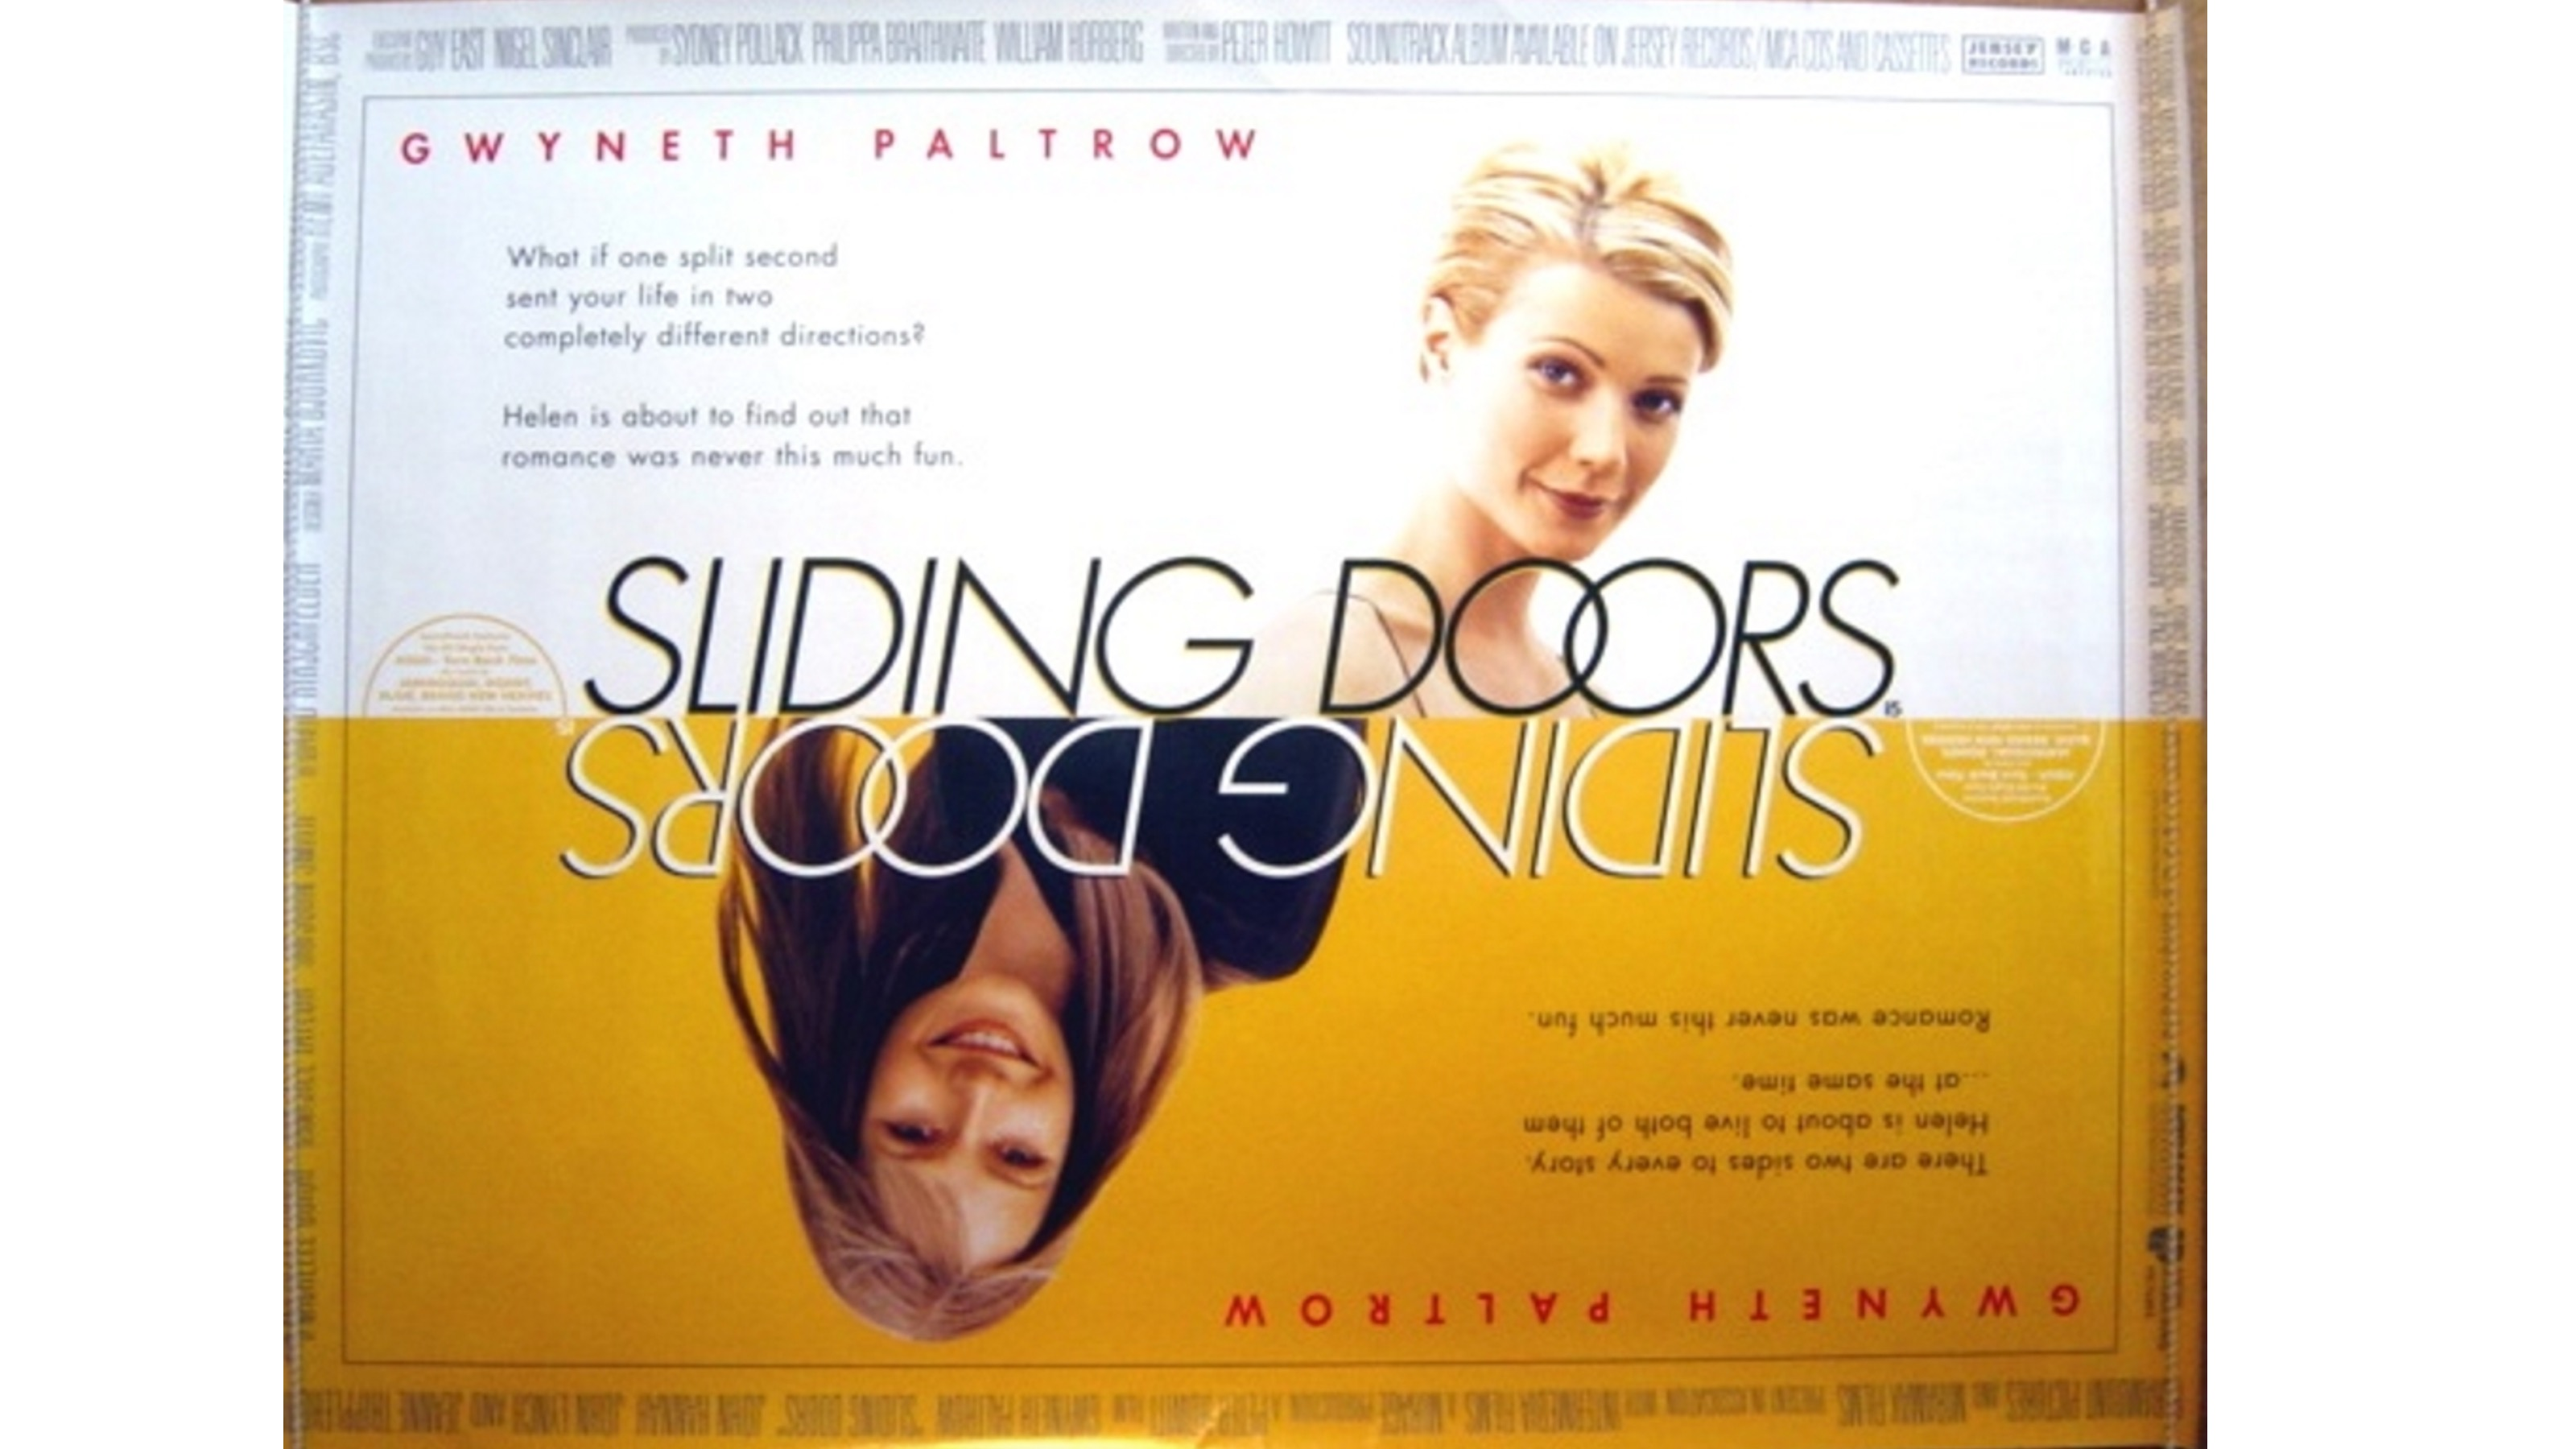
\includegraphics[keepaspectratio]{slidingdoors.jpg}}
\end{frame}

\begin{frame}{}
\phantomsection\label{section}
\pandocbounded{
\includegraphics[keepaspectratio]{frost.jpg}}
\end{frame}

\begin{frame}{\textbf{The Fundamental Problem of Causal Inference}}
\phantomsection\label{the-fundamental-problem-of-causal-inference}
To \textbf{quantify} a causal effect requires a \textbf{counterfactual}
contrast:

\[\tau_{you} = \Big[Y_{\text{you}}(a =1) - Y_{\text{you}}(a=0)\Big]\]

Where, \(Y(a)\) denotes the potential outcome under an intervention
\(A = a\). Here, we assume a binary intervention. At any time, we may
observe the outcome of only \textcolor{red}{one intervention, not both.}
\end{frame}

\begin{frame}{However, we only observe \emph{facts} not
\emph{counterfactuals}}
\phantomsection\label{however-we-only-observe-facts-not-counterfactuals}
\[
Y_i|A_i = 1 \implies Y_i(0)|A_i = 1~ \textcolor{red}{\text{is counterfactual}}
\]

``\textbf{And sorry I could not travel both. And be one traveller, long
I stood} \(\dots\)''
\end{frame}

\begin{frame}{Average Treatment Effect in randomised controlled
experiments work from assumptions}
\phantomsection\label{average-treatment-effect-in-randomised-controlled-experiments-work-from-assumptions}
\[
\text{Average Treatment Effect} = \left[ \begin{aligned}
&\left( \underbrace{\mathbb{E}[Y(1)|A = 1]}_{\text{observed}} + \textcolor{cyan}{\underbrace{\mathbb{E}[Y(1)|A = 0]}_{\text{unobserved}}} \right) \\
&- \left( \underbrace{\mathbb{E}[Y(0)|A = 0]}_{\text{observed}} + \textcolor{cyan}{\underbrace{\mathbb{E}[Y(0)|A = 1]}_{\text{unobserved}}} \right)
\end{aligned} \right]
\]
\end{frame}

\begin{frame}{Under identifying assumptions, we may infer causal effects
from associations}
\phantomsection\label{under-identifying-assumptions-we-may-infer-causal-effects-from-associations}
\[
\text{ATE} = \sum_{l} \left( \mathbb{E}[Y|A=1, \textcolor{cyan}{L=l}] - \mathbb{E}[Y|A=0, \textcolor{cyan}{L=l}] \right) \times \textcolor{cyan}{\Pr(L=l)}
\]

Where \(L\) is a set of measured covariates and \(A\coprod Y(a)|L\)
\end{frame}

\section{\texorpdfstring{\textbf{Part 2: The First Self-Inflicted Error:
The \emph{What}
Error}}{Part 2: The First Self-Inflicted Error: The What Error}}\label{part-2-the-first-self-inflicted-error-the-what-error}

\begin{frame}{Paradigmatic Concern: Confounding by Common Cause}
\phantomsection\label{paradigmatic-concern-confounding-by-common-cause}
\[\commoncauseT\]
\end{frame}

\begin{frame}{Where assumptions justify, we may condition on measured
confounders to obtain balance.}
\phantomsection\label{where-assumptions-justify-we-may-condition-on-measured-confounders-to-obtain-balance.}
\begin{columns}[T]
\begin{column}{0.5\linewidth}
\[
\commoncauseT
\]
\end{column}

\begin{column}{0.5\linewidth}
\[
\commoncausesolvedT
\]
\end{column}
\end{columns}
\end{frame}

\section{Error 1 -- What
(over-adjustment)}\label{error-1-what-over-adjustment}

\begin{frame}{``What Error \#1'': \textbf{Mediator Bias}}
\phantomsection\label{what-error-1-mediator-bias}
\[\mediatorT\]
\end{frame}

\begin{frame}[fragile]{Data Generating Process}
\phantomsection\label{data-generating-process}
\begin{Shaded}
\begin{Highlighting}[]
\FunctionTok{library}\NormalTok{(tidyverse)}

\FunctionTok{set.seed}\NormalTok{(}\DecValTok{123}\NormalTok{)                           }\CommentTok{\# reproducibility}
\NormalTok{n        }\OtherTok{\textless{}{-}} \DecValTok{1000}
\NormalTok{service  }\OtherTok{\textless{}{-}} \FunctionTok{rbinom}\NormalTok{(n, }\DecValTok{1}\NormalTok{, }\FloatTok{0.5}\NormalTok{)          }\CommentTok{\# A}
\NormalTok{wealth   }\OtherTok{\textless{}{-}} \DecValTok{2} \SpecialCharTok{*}\NormalTok{ service }\SpecialCharTok{+} \FunctionTok{rnorm}\NormalTok{(n)     }\CommentTok{\# L}
\NormalTok{charity  }\OtherTok{\textless{}{-}} \FloatTok{1.5} \SpecialCharTok{*}\NormalTok{ wealth }\SpecialCharTok{+} \FunctionTok{rnorm}\NormalTok{(n, }\AttributeTok{sd =} \FloatTok{1.5}\NormalTok{)  }\CommentTok{\# Y}

\NormalTok{sim1 }\OtherTok{\textless{}{-}} \FunctionTok{tibble}\NormalTok{(service, wealth, charity)}
\end{Highlighting}
\end{Shaded}
\end{frame}

\begin{frame}{Model comparison}
\phantomsection\label{model-comparison}
\begin{table}
\caption{Controlling for the mediator reverses the sign of the service
coefficient.}\tabularnewline

\fontsize{12.0pt}{14.4pt}\selectfont
\begin{tabular*}{\linewidth}{@{\extracolsep{\fill}}lcccccc}
\toprule
 & \multicolumn{3}{c}{Model A: Omit L} & \multicolumn{3}{c}{Model B: Control for L} \\ 
\cmidrule(lr){2-4} \cmidrule(lr){5-7}
\textbf{Characteristic} & \textbf{Beta} & \textbf{95\% CI} & \textbf{p-value} & \textbf{Beta} & \textbf{95\% CI} & \textbf{p-value} \\ 
\midrule\addlinespace[2.5pt]
service & 2.9 & 2.6, 3.2 & <0.001 & -0.27 & -0.53, -0.01 & 0.043 \\ 
wealth &  &  &  & 1.6 & 1.5, 1.7 & <0.001 \\ 
\bottomrule
\end{tabular*}
\begin{minipage}{\linewidth}
Abbreviation: CI = Confidence Interval\\
\end{minipage}
\end{table}
\end{frame}

\begin{frame}[fragile]{Which model looks better?}
\phantomsection\label{which-model-looks-better}
\begin{Shaded}
\begin{Highlighting}[]
\FunctionTok{library}\NormalTok{(performance)}

\FunctionTok{compare\_performance}\NormalTok{(fit\_adjust, fit\_omit, }\AttributeTok{rank =} \ConstantTok{TRUE}\NormalTok{)}
\end{Highlighting}
\end{Shaded}

\begin{verbatim}
# Comparison of Model Performance Indices

Name       | Model |    R2 | R2 (adj.) |  RMSE | Sigma | AIC weights
--------------------------------------------------------------------
fit_adjust |    lm | 0.682 |     0.682 | 1.473 | 1.475 |        1.00
fit_omit   |    lm | 0.312 |     0.311 | 2.169 | 2.171 |   2.88e-168

Name       | AICc weights | BIC weights | Performance-Score
-----------------------------------------------------------
fit_adjust |         1.00 |        1.00 |           100.00%
fit_omit   |    2.91e-168 |   3.35e-167 |             0.00%
\end{verbatim}

\begin{Shaded}
\begin{Highlighting}[]
\CommentTok{\# BIC(fit\_adjust) {-} BIC(fit\_omit)  \# negative → "better" fit}
\end{Highlighting}
\end{Shaded}
\end{frame}

\begin{frame}{``What Error \#2'': Collider Bias}
\phantomsection\label{what-error-2-collider-bias}
\[\colliderT\]
\end{frame}

\begin{frame}[fragile]{Data Generating Process}
\phantomsection\label{data-generating-process-1}
\begin{Shaded}
\begin{Highlighting}[]
\FunctionTok{set.seed}\NormalTok{(}\DecValTok{2025}\NormalTok{)}

\NormalTok{n          }\OtherTok{\textless{}{-}} \DecValTok{1000}
\NormalTok{service    }\OtherTok{\textless{}{-}} \FunctionTok{rbinom}\NormalTok{(n, }\DecValTok{1}\NormalTok{, }\FloatTok{0.5}\NormalTok{)                            }\CommentTok{\# A}
\NormalTok{donations  }\OtherTok{\textless{}{-}} \FunctionTok{rnorm}\NormalTok{(n)                                     }\CommentTok{\# Y}
\NormalTok{wealth     }\OtherTok{\textless{}{-}} \FunctionTok{rnorm}\NormalTok{(n, }\AttributeTok{mean =}\NormalTok{ service }\SpecialCharTok{+}\NormalTok{ donations, }\AttributeTok{sd =} \DecValTok{1}\NormalTok{) }\CommentTok{\# collider L}

\NormalTok{sim2 }\OtherTok{\textless{}{-}} \FunctionTok{tibble}\NormalTok{(service, wealth, donations)}
\end{Highlighting}
\end{Shaded}
\end{frame}

\begin{frame}{Model Comparison}
\phantomsection\label{model-comparison-1}
\begin{table}
\caption{Adding the collider creates a spurious, significant effect of A.}\tabularnewline

\fontsize{12.0pt}{14.4pt}\selectfont
\begin{tabular*}{\linewidth}{@{\extracolsep{\fill}}lcccccc}
\toprule
 & \multicolumn{3}{c}{Model A: Omit L} & \multicolumn{3}{c}{Model B: Control for L (collider)} \\ 
\cmidrule(lr){2-4} \cmidrule(lr){5-7}
\textbf{Characteristic} & \textbf{Beta} & \textbf{95\% CI} & \textbf{p-value} & \textbf{Beta} & \textbf{95\% CI} & \textbf{p-value} \\ 
\midrule\addlinespace[2.5pt]
service & 0.00 & -0.12, 0.13 & >0.9 & -0.53 & -0.63, -0.44 & <0.001 \\ 
wealth &  &  &  & 0.51 & 0.48, 0.54 & <0.001 \\ 
\bottomrule
\end{tabular*}
\begin{minipage}{\linewidth}
Abbreviation: CI = Confidence Interval\\
\end{minipage}
\end{table}
\end{frame}

\begin{frame}[fragile]{Which model looks better?}
\phantomsection\label{which-model-looks-better-1}
\begin{Shaded}
\begin{Highlighting}[]
\FunctionTok{compare\_performance}\NormalTok{(fit\_biased, fit\_correct, }\AttributeTok{rank =} \ConstantTok{TRUE}\NormalTok{)}
\end{Highlighting}
\end{Shaded}

\begin{verbatim}
# Comparison of Model Performance Indices

Name        | Model |        R2 |  R2 (adj.) |  RMSE | Sigma | AIC weights
--------------------------------------------------------------------------
fit_biased  |    lm |     0.526 |      0.525 | 0.707 | 0.708 |        1.00
fit_correct |    lm | 3.722e-06 | -9.983e-04 | 1.028 | 1.029 |   1.42e-162

Name        | AICc weights | BIC weights | Performance-Score
------------------------------------------------------------
fit_biased  |         1.00 |        1.00 |           100.00%
fit_correct |    1.43e-162 |   1.65e-161 |             0.00%
\end{verbatim}

\begin{Shaded}
\begin{Highlighting}[]
\FunctionTok{BIC}\NormalTok{(fit\_biased) }\SpecialCharTok{{-}} \FunctionTok{BIC}\NormalTok{(fit\_correct)}
\end{Highlighting}
\end{Shaded}

\begin{verbatim}
[1] -740.425
\end{verbatim}
\end{frame}

\begin{frame}{Take-Home}
\phantomsection\label{take-home}
\begin{tcolorbox}[enhanced jigsaw, breakable, opacityback=0, opacitybacktitle=0.6, toprule=.15mm, colbacktitle=quarto-callout-important-color!10!white, colframe=quarto-callout-important-color-frame, bottomtitle=1mm, titlerule=0mm, colback=white, bottomrule=.15mm, arc=.35mm, leftrule=.75mm, coltitle=black, toptitle=1mm, title=\textcolor{quarto-callout-important-color}{\faExclamation}\hspace{0.5em}{Important}, rightrule=.15mm, left=2mm]

Relying on model fit perpetuates the \emph{causality crisis} in
psychology (\citeproc{ref-bulbulia2022}{Bulbulia 2023}).\\
Draw the DAG first; decide what belongs in the model before looking at
numbers.

\end{tcolorbox}
\end{frame}

\begin{frame}{The What Error is widespread in \textbf{experimental}
studies in the social sciences}
\phantomsection\label{the-what-error-is-widespread-in-experimental-studies-in-the-social-sciences}
\begin{itemize}
\item
  ``Overall, we find that \textbf{46.7\% of the experimental studies}
  published in APSR, AJPS, and JOP from 2012 to 2014 engaged in
  posttreatment conditioning (35 of 75 studies) \ldots{}''
\item
  ``About \textbf{1 in 4 drop cases or subset the data based on
  post-treatment criteria,} and \textbf{nearly a third include
  post-treatment variables as covariates}''
\item
  ``Most tellingly, \textbf{nearly 1 in 8 articles directly conditions
  on variables that the authors themselves show as being an outcome of
  the experiment} -- an unambiguous indicator of \textbf{a fundamental
  lack of understanding \ldots{} that conditioning on posttreatment
  variables can invalidate results from randomized experiments.}''
\item
  ``Empirically, then, the answer to the question of \textbf{whether the
  discipline already understands posttreatment bias is clear: It does
  not.}'' (\citeproc{ref-montgomery2018}{Montgomery, Nyhan, and Torres
  2018})
\end{itemize}
\end{frame}

\begin{frame}{Mediator Bias control strategy: \textbf{Longitudinal
Hygiene}}
\phantomsection\label{mediator-bias-control-strategy-longitudinal-hygiene}
\begin{columns}[T]
\begin{column}{0.5\linewidth}
\[
\mediatorT
\]
\end{column}

\begin{column}{0.5\linewidth}
\[
\commoncausesolvedT
\]
\end{column}
\end{columns}
\end{frame}

\begin{frame}{How to Tame The What Error? \textbf{Hide your future}}
\phantomsection\label{how-to-tame-the-what-error-hide-your-future}
Use Repeated Measures on the Same Individuals
\end{frame}

\begin{frame}{Collider bias control strategy: \textbf{Hide your future}}
\phantomsection\label{collider-bias-control-strategy-hide-your-future}
\begin{columns}[T]
\begin{column}{0.5\linewidth}
\[\colliderT\]
\end{column}

\begin{column}{0.5\linewidth}
\[\commoncausesolvedT\]
\end{column}
\end{columns}
\end{frame}

\begin{frame}{Collider bias by proxy control strategy: \textbf{Hide your
future}}
\phantomsection\label{collider-bias-by-proxy-control-strategy-hide-your-future}
\begin{columns}[T]
\begin{column}{0.5\linewidth}
\[\commoncausechildT\]
\end{column}

\begin{column}{0.5\linewidth}
\[\commoncausesolvedchildT\]
\end{column}
\end{columns}
\end{frame}

\begin{frame}{Post-exposure collider bias control strategy: \textbf{Hide
your future}}
\phantomsection\label{post-exposure-collider-bias-control-strategy-hide-your-future}
\begin{columns}[T]
\begin{column}{0.5\linewidth}
\[\mediatorcolliderT\]
\end{column}

\begin{column}{0.5\linewidth}
\[\commoncausesolvedT\]
\end{column}
\end{columns}
\end{frame}

\begin{frame}{Finally, our biggest worry: \textbf{Unmeasured Common
Causes}}
\phantomsection\label{finally-our-biggest-worry-unmeasured-common-causes}
\[\downstreamT\]
\end{frame}

\begin{frame}{Unmeasured common cause strategy: \textbf{Hide your
future}}
\phantomsection\label{unmeasured-common-cause-strategy-hide-your-future}
\begin{columns}[T]
\begin{column}{0.5\linewidth}
\[\downstreamT\]
\end{column}

\begin{column}{0.5\linewidth}
\[\commoncausesolvedT\]
\end{column}
\end{columns}

And because \textcolor{cyan}{hope is not enough}, we should consistently
report sensitivity analyses.
\end{frame}

\begin{frame}{Are longitudinal data + sensitivity analysis enough?}
\phantomsection\label{are-longitudinal-data-sensitivity-analysis-enough}
\begin{columns}[T]
\begin{column}{0.5\linewidth}
If the data we collect were like this:
\[Y_{\text{time 0}} ~~...~~ A_{\text{time 1}}\]
\end{column}

\begin{column}{0.5\linewidth}
We should not be tempted to model this.

\[\ytoacrazyT\]
\end{column}
\end{columns}
\end{frame}

\begin{frame}{Are longitudinal data + sensitivity analysis enough?}
\phantomsection\label{are-longitudinal-data-sensitivity-analysis-enough-1}
\textcolor{cyan}{Too obvious} this is wrong?

\[\ytoacrazyT\]
\end{frame}

\section{Error 2: When (time-zero)}\label{error-2-when-time-zero}

\begin{frame}{\textbf{Longitudinal data} are \textbf{not} enough}
\phantomsection\label{longitudinal-data-are-not-enough}
Temporal ordering was \textcolor{cyan}{precisely the problem} with the
observational hormone studies in the 80s/90s that modelled
\textcolor{cyan}{longitudinal data}.

\textbf{How?}
\end{frame}

\begin{frame}{Researchers failed to emulate an experiment in their data
(Target Trial)}
\phantomsection\label{researchers-failed-to-emulate-an-experiment-in-their-data-target-trial}
\begin{itemize}
\item
  Women's Health Initiative: overall hazard ratio 1.23 (0.99, 1.53)
\item
  Women's Health Initiative: when broken down by years to follow-up:

  \begin{itemize}
  \tightlist
  \item
    0-2 years 1.51 (1.06, 2.14)
  \item
    2-5 years 1.31 (0.93, 1.83)
  \item
    5 or more years \textbf{0.67 (0.41, 1.09)}
  \end{itemize}
\end{itemize}

\begin{tcolorbox}[enhanced jigsaw, breakable, opacityback=0, opacitybacktitle=0.6, toprule=.15mm, colbacktitle=quarto-callout-note-color!10!white, colframe=quarto-callout-note-color-frame, bottomtitle=1mm, titlerule=0mm, colback=white, bottomrule=.15mm, arc=.35mm, leftrule=.75mm, coltitle=black, toptitle=1mm, title={Survivor Bias.}, rightrule=.15mm, left=2mm]

The observational results can be
\textcolor{cyan}{entirely explained by selection bias}

\end{tcolorbox}

\begin{tcolorbox}[enhanced jigsaw, breakable, opacityback=0, opacitybacktitle=0.6, toprule=.15mm, colbacktitle=quarto-callout-note-color!10!white, colframe=quarto-callout-note-color-frame, bottomtitle=1mm, titlerule=0mm, colback=white, bottomrule=.15mm, arc=.35mm, leftrule=.75mm, coltitle=black, toptitle=1mm, title={Emulating a target trial with observational data recovers experimental
effects.}, rightrule=.15mm, left=2mm]

Re-modelling \textcolor{cyan}{initiation into hormone therapy} recovers
experimental findings (\citeproc{ref-hernan2016}{Hernán et al. 2016}).

\end{tcolorbox}
\end{frame}

\begin{frame}{Visualising the When Error}
\phantomsection\label{visualising-the-when-error}
\begin{figure}

\centering{

\pandocbounded{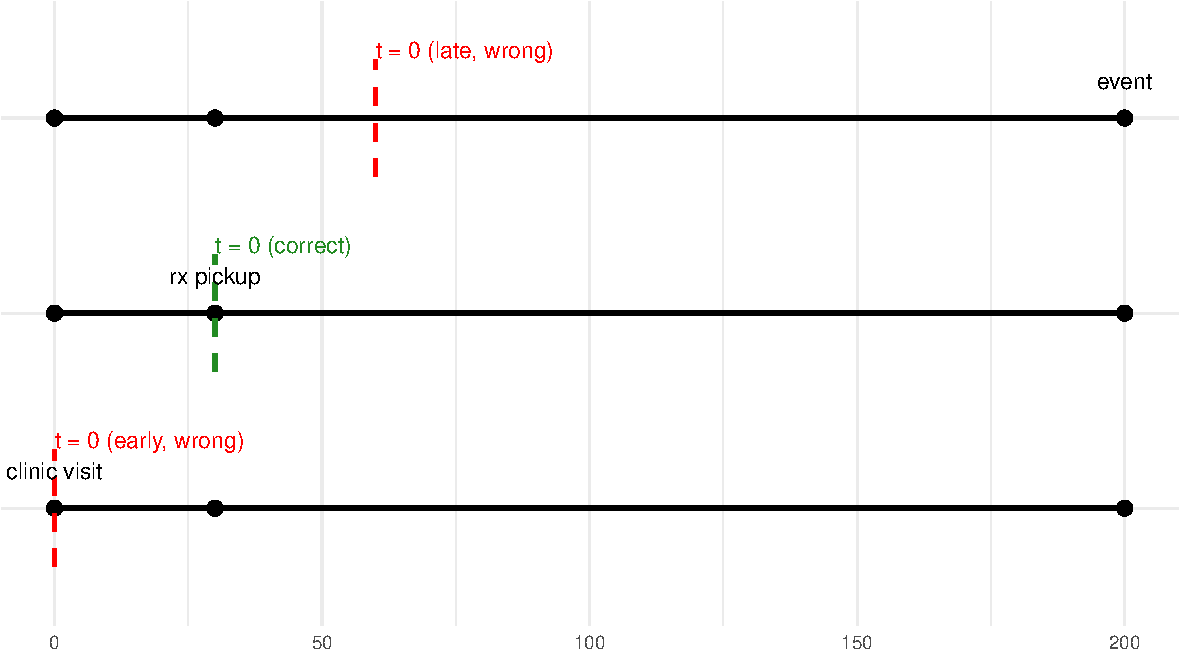
\includegraphics[keepaspectratio]{talking-points_files/figure-beamer/fig-time-zero-3lines-1.pdf}}

}

\caption{\label{fig-time-zero-3lines}Three ways to start the clock. Only
one is right.}

\end{figure}%
\end{frame}

\begin{frame}{Target Trial Check List}
\phantomsection\label{target-trial-check-list}
\begin{table}

\caption{\label{tbl-target-trial}Target-trial specification for the
hormone-therapy example.}

\centering{

\centering
\begin{tabular}[t]{ll}
\toprule
element & definition\\
\midrule
\cellcolor{gray!10}{Eligibility} & \cellcolor{gray!10}{Post-menopausal women aged 50–79, no prior CHD}\\
Treatment & Initiate oestrogen + progestin on day of Rx pickup\\
\cellcolor{gray!10}{Comparison} & \cellcolor{gray!10}{No hormone-therapy initiation on that day}\\
Outcome & All-cause mortality\\
\cellcolor{gray!10}{Follow-up} & \cellcolor{gray!10}{8 years or until death / loss to follow-up}\\
\bottomrule
\end{tabular}

}

\end{table}%
\end{frame}

\section{Error 3 -- Who (population and
heterogeneity)}\label{error-3-who-population-and-heterogeneity}

\begin{frame}{Illustration}
\phantomsection\label{illustration}
\end{frame}

\section{New Zealand Attitudes and Values Study (NZAVS): A step-by-step
workflow for causal
inference}\label{new-zealand-attitudes-and-values-study-nzavs-a-step-by-step-workflow-for-causal-inference}

\begin{frame}{The New Zealand Attitudes and Values Study:}
\phantomsection\label{the-new-zealand-attitudes-and-values-study}
\begin{itemize}
\item
  Planned 20-year longitudinal study, currently in its 14th year,
  \textgreater{} 77k measured
\item
  Sample frame is drawn randomly from the NZ Electoral Roll.
\end{itemize}
\end{frame}

\begin{frame}{Causal Questions}
\phantomsection\label{causal-questions}
\begin{enumerate}
[1)]
\item
  Average Treatment Effect: Difference in averages of social outcomes
  (a) if everyone in New Zealand were to attend religious service at
  least 1x per month (b) if everyone were not to attend religious
  service at all.
\item
  Heterogeneous Treatment Effects: Machine learning of groups who differ
  in such effects. Focus here on Qini Curve at 20\% and 30\% of full
  ``budget''.
\item
  Use Qini results to select for Policy Trees: Clarify \emph{who}
  responds strongly/weakly.
\end{enumerate}

\textbf{Note: all results use ``honest'' learning -- sample is split
into training/test sets (here 70/30).}
\end{frame}

\begin{frame}{Outcomes}
\phantomsection\label{outcomes}
\begin{enumerate}
\tightlist
\item
  Sense of Belonging
\item
  Social Support
\item
  Charitable Donations (annual)
\item
  Volunteering (weekly)
\end{enumerate}

\textbf{All outcomes measured one year after the intervention}
\end{frame}

\begin{frame}{Three-wave Panel Design: control for baseline exposure and
outcome among confounder set.}
\phantomsection\label{three-wave-panel-design-control-for-baseline-exposure-and-outcome-among-confounder-set.}
\[
\threeLONG
\]
\end{frame}

\begin{frame}{Target Population: Residents of New Zealand in 2018 had
they not been censored through 2021.}
\phantomsection\label{target-population-residents-of-new-zealand-in-2018-had-they-not-been-censored-through-2021.}
\begin{block}{Census Weights (Age X Gender X Ethnicity)}
\phantomsection\label{census-weights-age-x-gender-x-ethnicity}
\pandocbounded{\includegraphics[keepaspectratio]{hist_sample_weights.png}}
\end{block}

\begin{block}{(IPCW Stabilised \& Trimmed)}
\phantomsection\label{ipcw-stabilised-trimmed}
\pandocbounded{\includegraphics[keepaspectratio]{hist_combo_weights.png}}
\end{block}
\end{frame}

\begin{frame}{Religious Service Intervention}
\phantomsection\label{religious-service-intervention}
\[f(A) = \begin{cases} 1 & \text{if } a \ge 0 \text{ At least 1 x per month Religious Attendance} \\ 0 & \text{if } a = 0 \text{ Monthly Religious Service} \end{cases}\]
\end{frame}

\begin{frame}{Histogram Showing Split}
\phantomsection\label{histogram-showing-split}
\pandocbounded{\includegraphics[keepaspectratio]{2025_church_graph_cut.png}}
\end{frame}

\begin{frame}{Love Plot of Propensity Scores}
\phantomsection\label{love-plot-of-propensity-scores}
\pandocbounded{\includegraphics[keepaspectratio]{2025_church_propensity.png}}
\end{frame}

\begin{frame}{Average Treatment Effect Results:}
\phantomsection\label{average-treatment-effect-results}
\end{frame}

\begin{frame}{Workflow}
\phantomsection\label{workflow}
\begin{itemize}
\tightlist
\item
  Target population: New Zealand Population by 2018 census weights
\item
  Outcomes: all NZAVS outcomes relating to pro-sociality (outcome-wide
  study)
\item
  Missing data: inverse-probability of censoring weights
  non-parametrically estimated/ causal forests permit missing data at
  baseline
\item
  Eligibility: participated in NZAVS 2018 (wave-10) and 2019 (wave 11,
  exposure wave) may have been lost to follow-up in wave 12,
  \textbf{46,377}.
\item
  Bonferroni correct for multiple comparisons / E-value threshold = 1.2
\end{itemize}
\end{frame}

\begin{frame}{Transition table: Religious Attendance}
\phantomsection\label{transition-table-religious-attendance}
\begin{longtable}[]{@{}lrrr@{}}
\toprule\noalign{}
From / To & State 0 & State 1 & Total \\
\midrule\noalign{}
\endhead
State 0 & 28545 & 681 & 29226 \\
State 1 & 887 & 3593 & 4480 \\
\bottomrule\noalign{}
\end{longtable}
\end{frame}

\begin{frame}{Average Treatment Effect}
\phantomsection\label{average-treatment-effect}
The following outcomes showed reliable causal evidence (E‑value lower
bound \textgreater{} 1.2): - Volunteering (weekly, log):
0.154(0.056,0.252); on the original scale, 11.264 minutes(3.943,19.158).
E‑value bound = 1.287 - log Charity Donate: 0.13(0.045,0.215); on the
original scale, 39.935 (12.247,74.883). E‑value bound = 1.25
\end{frame}

\section{Graph ATE}\label{graph-ate}

\begin{frame}{Graph ATE}
\pandocbounded{\includegraphics[keepaspectratio]{2025_church_ate.png}}
\end{frame}

\begin{frame}{How Much Better if We Treated by CATE?}
\phantomsection\label{how-much-better-if-we-treated-by-cate}
\pandocbounded{\includegraphics[keepaspectratio]{2025_church_combined_qini.png}}
\end{frame}

\begin{frame}{Who Should We Treat First? Belonging}
\phantomsection\label{who-should-we-treat-first-belonging}
\pandocbounded{\includegraphics[keepaspectratio]{2025_2L_church_on_belonging.png}}
\end{frame}

\begin{frame}{Who Should We Treat First? Charitable Donations}
\phantomsection\label{who-should-we-treat-first-charitable-donations}
\pandocbounded{\includegraphics[keepaspectratio]{2025_2L_church_on_charity_donations.png}}
\end{frame}

\begin{frame}{Closing}
\phantomsection\label{closing}
\begin{longtable}[]{@{}
  >{\raggedright\arraybackslash}p{(\linewidth - 4\tabcolsep) * \real{0.1134}}
  >{\raggedright\arraybackslash}p{(\linewidth - 4\tabcolsep) * \real{0.3505}}
  >{\raggedright\arraybackslash}p{(\linewidth - 4\tabcolsep) * \real{0.5361}}@{}}
\toprule\noalign{}
\begin{minipage}[b]{\linewidth}\raggedright
\textbf{Error}
\end{minipage} & \begin{minipage}[b]{\linewidth}\raggedright
\textbf{Need}
\end{minipage} & \begin{minipage}[b]{\linewidth}\raggedright
\textbf{Remedy}
\end{minipage} \\
\midrule\noalign{}
\endhead
What & Control the right variables & Draw a DAG first \\
When & Start the clock on time & Emulate a target trial \\
Who & Treat the right people & Weight to target + investigate
heterogeneity \\
\bottomrule\noalign{}
\end{longtable}
\end{frame}

\begin{frame}{Thanks}
\phantomsection\label{thanks}
\begin{itemize}
\tightlist
\item
  TRT Grant 0418 \& Max Planck Institute for Evolutionary Anthropology
  for support.
\item
  Chris G. Sibley (NZAVS lead Investigator) for the heavy data lifting
\item
  77,490 NZAVS participants for their time
\item
  \textcolor{cyan}{Reach out} with questions or if you would like to
  become involved:
  \href{emailto:joseph.bulbulia@vuw.ac.nz}{joseph.bulbulia@vuw.ac.nz}
\end{itemize}
\end{frame}

\begin{frame}
\begin{figure}[H]

{\centering \pandocbounded{\includegraphics[keepaspectratio]{NZAVS-QR.png}}

}

\caption{NZAVS}

\end{figure}%
\end{frame}

\begin{frame}{}
\phantomsection\label{section-1}
\phantomsection\label{refs}
\begin{CSLReferences}{1}{0}
\bibitem[\citeproctext]{ref-bulbulia2022}
Bulbulia, Joseph A. 2023. {``A Workflow for Causal Inference in
Cross-Cultural Psychology.''} \emph{Religion, Brain \& Behavior} 13 (3):
291--306. \url{https://doi.org/10.1080/2153599X.2022.2070245}.

\bibitem[\citeproctext]{ref-grodstein2006hormone}
Grodstein, Francine, Joann E Manson, and Meir J Stampfer. 2006.
{``Hormone Therapy and Coronary Heart Disease: The Role of Time Since
Menopause and Age at Hormone Initiation.''} \emph{Journal of Women's
Health} 15 (1): 35--44.

\bibitem[\citeproctext]{ref-hernan2016}
Hernán, Miguel A, Brian C Sauer, Sonia Hernández-Díaz, Robert Platt, and
Ian Shrier. 2016. {``Specifying a Target Trial Prevents Immortal Time
Bias and Other Self-Inflicted Injuries in Observational Analyses.''}
\emph{Journal of Clinical Epidemiology} 79: 70--75.

\bibitem[\citeproctext]{ref-manson2003estrogen}
Manson, JoAnn E, Judith Hsia, Karen C Johnson, Jacques E Rossouw,
Annlouise R Assaf, Norman L Lasser, Maurizio Trevisan, et al. 2003.
{``Estrogen Plus Progestin and the Risk of Coronary Heart Disease.''}
\emph{New England Journal of Medicine} 349 (6): 523--34.

\bibitem[\citeproctext]{ref-montgomery2018}
Montgomery, Jacob M., Brendan Nyhan, and Michelle Torres. 2018. {``How
Conditioning on Posttreatment Variables Can Ruin Your Experiment and
What to Do about It.''} \emph{American Journal of Political Science} 62
(3): 760--75. \url{https://doi.org/10.1111/ajps.12357}.

\end{CSLReferences}
\end{frame}




\end{document}
